\documentclass{beamer}
\usetheme[]{Boadilla}

\usepackage{float}
\usepackage{graphicx}
\usepackage{subfig}

\title{Logical Neural Networks}
\subtitle{Opening The Black Box\\
\vspace{0.5cm}
\small COMP 489 Project
}
\author{Daniel Braithwaite}
\date{Supervisor: Marcus Frean}

\begin{document}

\begin{frame}
\titlepage
\end{frame}

\begin{frame}
\frametitle{Introduction + Motivation}

\begin{figure}
\centering
	\begin{minipage}[b]{0.8\textwidth}
		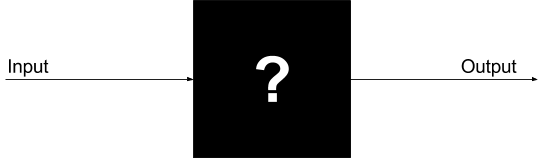
\includegraphics[width=\textwidth]{Images/BlackBox.png}
	\end{minipage}
	\hfill
\end{figure}

Diffcult to intepret Artificial Neural Networks using standard activations, e.g., Sigmoid, TanH.

\begin{block}{Why Intepretable Systems?}
\begin{itemize}
\item Saftey Critical Systems
\item Ensuring systems make Ethical decisions
\item European Union General Data Protection Regulation
\end{itemize}
\end{block}
\end{frame}

\begin{frame}
\frametitle{Problem Statement}

Want ANNs which not only achieve high accuracy but have logic that can be defended.

\end{frame}

\begin{frame}
\frametitle{Idea}

\begin{itemize}
\item Some problems appear to have a logic decomposition 
\item Logical functions are easy for humans to intepret
\item \textbf{Goal:} Learn these logical decompositions using backpropergation
\item \textbf{Problem:} Standard Boolean Logic Gates are not continous.
\end{itemize}

\end{frame}

\begin{frame}
\frametitle{Noisy Neurons}

\begin{figure}
\centering
	\begin{minipage}[b]{0.4\textwidth}
		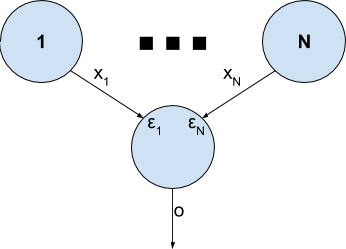
\includegraphics[width=\textwidth]{Images/NoisyNeuronEG.png}
	\end{minipage}
	\hfill
\end{figure}

\begin{itemize}
\item They represent a continous paramaterisation of descrete logic gates.
\item $x_i$ is probability the $i$'th input is on.
\item $\epsilon_i$ is the probability that input $i$ is irrelevent. The $\epsilon$'s are the learned weights
\item There exsists Noisy-AND and Noisy-OR Neurons.
\end{itemize}


\end{frame}

\begin{frame}
\frametitle{Approach: Logical Neural Networks}
Logical Neural Networks have layers consisting of Noisy Neurons. Can be trained with backpropagation.

\begin{block}{Problem: Weight Initlization}
\begin{itemize}
\item Even small networks wouldent train.
\item Derived a distrubution from which to sample weights.
\item Now large networks can be trained, inluding deep Logical Networks. Up-to 10 layers deep!
\end{itemize}
\end{block}

\end{frame}

\begin{frame}
\frametitle{Experemental Approach}

\begin{itemize}
\item Want to evaluate accuracy and peformance of Logical Neural Networks
\item Will use MNIST problem.
\item \textbf{Peformance:} Networks trained from 30 different initial conditions, peformance compared using confidence intervals from evaluation of network on testing set.
\item \textbf{Intepretability:} Diffcult to establish. Results are obtained by visually comparing intepretations of the weights from different networks.
\end{itemize}
\end{frame}

\begin{frame}
\frametitle{Experemental Results: Performance}

\begin{itemize}
\item Logical Neural Networks have stistically equivelent peformance to Multi-Layer Perceptron Networks.
\end{itemize}
\end{frame}

\begin{frame}
\frametitle{Experemental Results: Intepretability}
\begin{itemize}
\item Logical Neural Networks are potentially more intepretable that Multi-Layer Perceptron Networks.
\item Intepretability of Logical Neural Networks depends on activations used.
\end{itemize}
\end{frame}

\begin{frame}
\frametitle{Experemental Results: Intepretability - No Hidden}
%\begin{example}{Single Layer Networks}

%\begin{itemize}
%\item Perceptron Network
\begin{minipage}[t]{0.4\textwidth}
\begin{figure}[H]
	\centering
	\begin{minipage}[b]{0.7\textwidth}
		\captionsetup{labelformat=empty}
		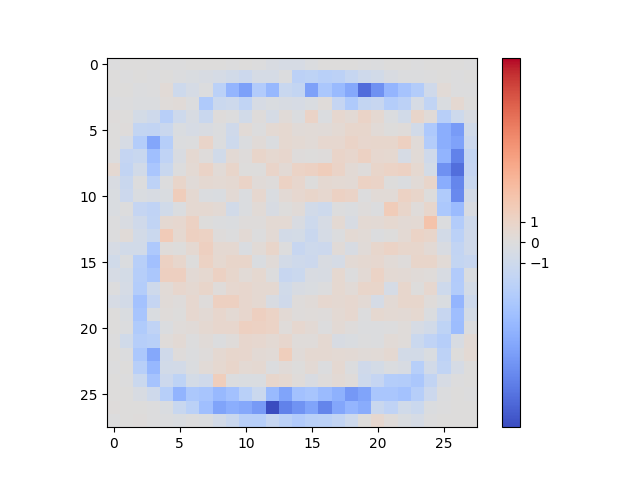
\includegraphics[width=\textwidth]{Images/Sigmoid(NO-Hidden)/Layer0-Neuron-0.png}
		%\caption{Digit 0}
	\end{minipage}
	\caption{Features for a perceptron network}
	\hfill
\end{figure}
\end{minipage}
\hspace{0.1\textwidth}
\begin{minipage}[t]{0.4\textwidth}
\begin{figure}[H]
	%\captionsetup{labelformat=empty}
	\centering
	\begin{minipage}[b]{0.7\textwidth}
		\captionsetup{labelformat=empty}
		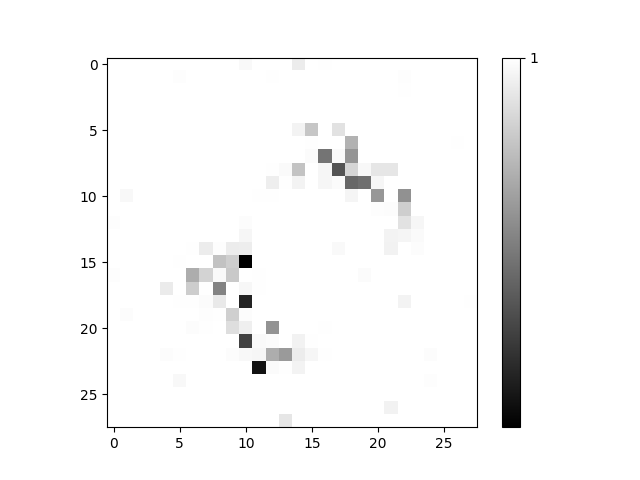
\includegraphics[width=\textwidth]{Images/AND(LSM)/Positive/Layer0-Neuron-0.png}
		%\caption{Digit 0}
	\end{minipage}
	
	\medskip

	\begin{minipage}[b]{0.7\textwidth}
		\captionsetup{labelformat=empty}
		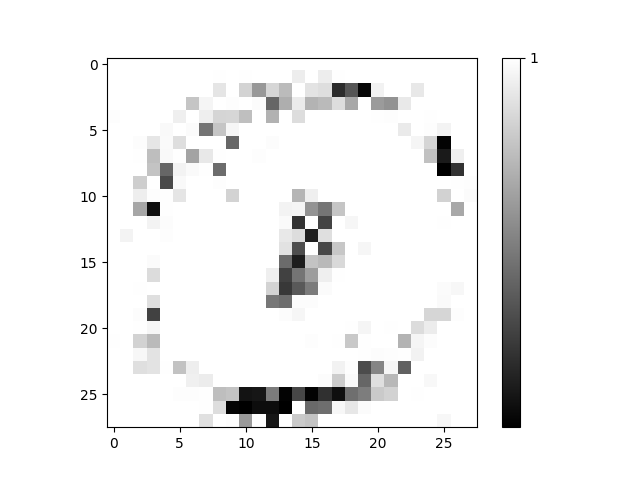
\includegraphics[width=\textwidth]{Images/AND(LSM)/Negative/Layer0-Neuron-0.png}
		%\caption{Not Digit 0}
	\end{minipage}
	\caption{Features for a logical neural network using an AND activation}
	\hfill
\end{figure}
\end{minipage}
%\end{itemize}

%\end{example}
\end{frame}

\begin{frame}
\frametitle{Experemental Results: Intepretability - Hidden Layers}

\noindent
\begin{minipage}[t]{0.4\textwidth}
	\begin{figure}[H]
		\centering
		\begin{minipage}[b]{0.7\textwidth}
			\captionsetup{labelformat=empty}
			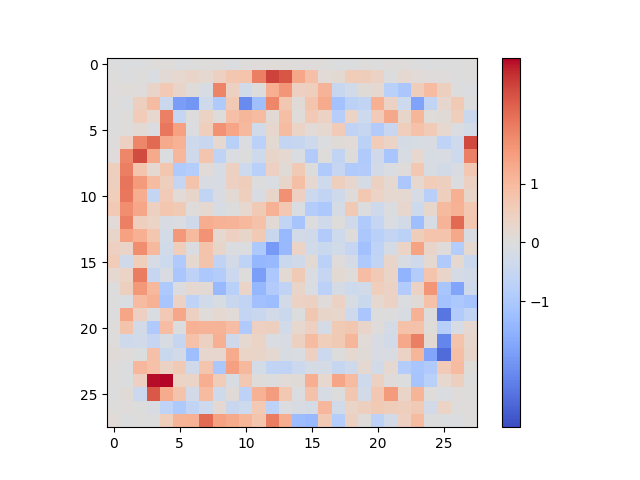
\includegraphics[width=\textwidth]{Images/Sigmoid(Hidden-Layer)/Like/Layer0-Neuron-11.png}
			%\caption{Digit 0}
			\label{}
		\end{minipage}
		\caption{Features that positively contribute to the classification as a 1.}
		\hfill
	\end{figure}
\end{minipage}
\hspace{0.1\textwidth}
\begin{minipage}[t]{0.4\textwidth}
\begin{figure}[H]
		\centering
		\begin{minipage}[b]{0.7\textwidth}
			\captionsetup{labelformat=empty}
			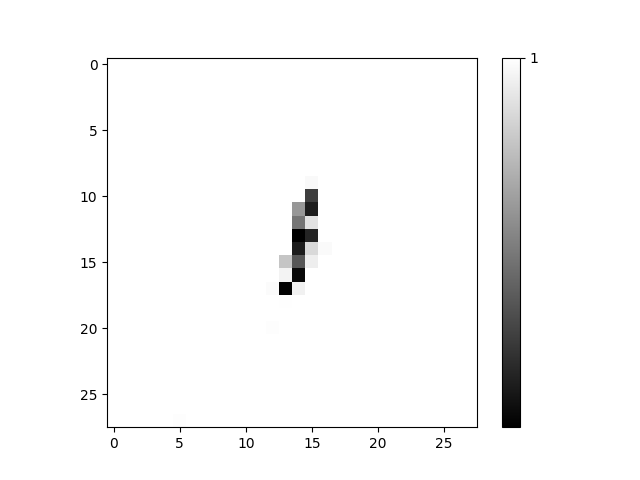
\includegraphics[width=\textwidth]{Images/AND-OR(W-LSM)(1)/Like/True/Layer0-Neuron-9.png}
			%\caption{Digit 0}
			\label{}
		\end{minipage}
		
		\medskip
		
		\begin{minipage}[b]{0.7\textwidth}
			\captionsetup{labelformat=empty}
			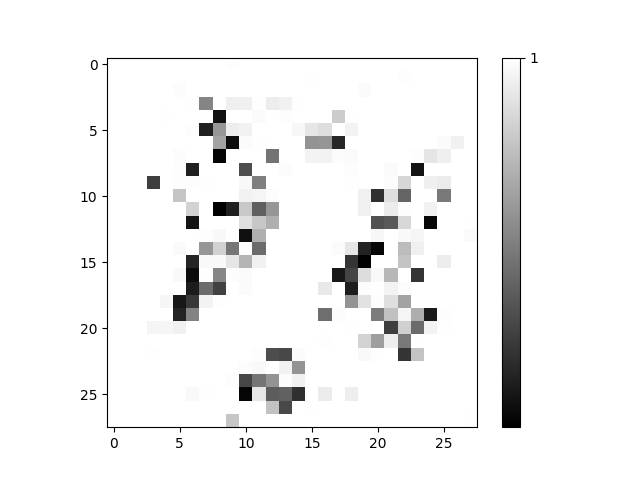
\includegraphics[width=\textwidth]{Images/AND-OR(W-LSM)(1)/Like/False/Layer0-Neuron-9.png}
			%\caption{Digit 0}
			\label{}
		\end{minipage}
		\caption{Features contributing to classification of a 1 in an  AND $\rightarrow$ OR Model}
		\hfill
	\end{figure}

\end{minipage}
\end{frame}

\begin{frame}
\frametitle{Conclusion}

\begin{block}{Did we succeed in solving the problem? Well... Yes and No}
\begin{itemize}
\item Logical Neural Networks are a promsing alternative to Multi-Layer Perceptron Networks.
\item Intepretability on MNIST was "better". But again, diffcult to establish.
\item Was found that intepreting Logical Neural Networks became diffcult with multiple layers.
\end{itemize}
\end{block}
\end{frame}

\begin{frame}
\begin{center}
\huge Questions
\end{center}
\end{frame}

\end{document}